\section{Comparaison avec la photo
terne}\label{comparaison-avec-la-photo-terne}

\begin{figure}[htbp]
\centering
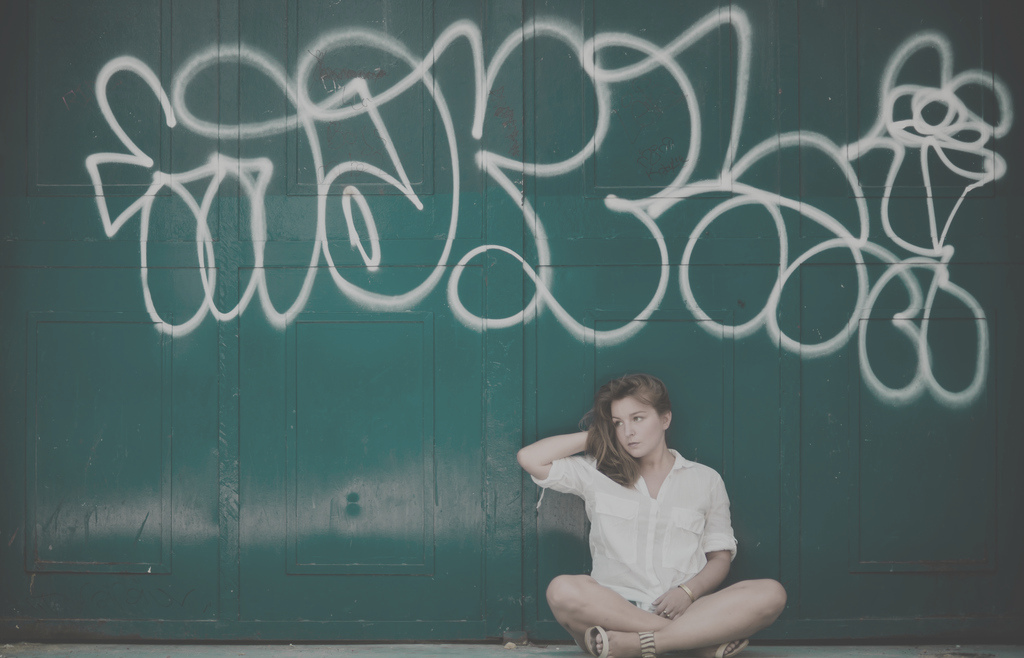
\includegraphics{../../photos/terne.jpg}
\caption{Photo terne}
\end{figure}

\begin{table}[htbp]
\centering
\begin{tabular}{llr}
\bfseries Formes (\%)&
\bfseries Bhattacharyya (\%)%
\DTLforeach*[\DTLiseq{\fichier}{photos/terne.jpg}]{valeurs}{%
\fichier=Fichier, \formes=Formes,\bhatta=Bhattacharyya, \hue=Hue, \saturation=Saturation, \value=Value}{%
\\
\formes & \bhatta}
\end{tabular}
\end{table}

Cette modification a un gros impact sur la photo originale, surtout au niveau
des couleurs.

On observe en effet $71.67 \%$ de différence au niveau colorimétrique et
$27.33 \%$ de différence au niveau des formes. On peut observer sur la photo
directement que toutes les couleurs ont changées ce qui explique les
$71.67 \%$. Les $27.33 \%$ des formes sont dues aux bordures que ce filtre doit
atténuer.
